\chapter{Dokumentacja techniczna}% 
Z racji tego że platforma ma obsługiwać zarówno wysokopoziomowe funkcje jak i niskopoziomowe jak GPIO w urządzeniu to projekt został podzielony na 2 części czyli część serwerową i stronę internetową. W tym rozdziale zostały opisane tylko istotne  części projektu które rozwiązują istotne problemy lub prezentują organizację kodu. Cały projekt został napisany według zasad opisanych w książce Clean Code gdzie jednym z ważniejszych zasad jest brak komentowania kodu. Kod sam siebie powinien opisywać za pomocą swojego nazewnictwa i struktury.  \cite{cleancode}
\section{Aplikacja internetowa}
Przy pomocy strony użytkownik monitoruje i steruje wszystkimi podłączonymi urządzeniami w budynku. Może także zobaczyć informacje pochodzące z czujników w domu np. pomiar temperatury w kuchni. \\
Projekt jest napisany w języku javascript ES6+ więc podczas rozwijania aplikacji internetowej posiłkujemy się transpilerem który konwertuje kod na starsze wersje javascript które są wspierane przez przeglądarki. Z tego powodu gdy tworzymy wersję produkcyjną musimy zbudować stronę, a następnie zaimportować do serwera. Ten aspekt będzie dalej opisywany w części serwerowej.
\par Istotnym aspektem aplikacji jest komunikacja z serwerem. jest ona nawiązywana na 2 etapowo.
Serwer ma wyprowadzony endpoint z którym łączy się strona celem otrzymania portu na którym działa websocket
\ref{lst:websocketGet}. W trakcie kiedy jeszcze czekamy na otrzymania odpowiedzi od serwera, kolejkujemy akcje które powinny być wysłane przez websocket \ref{lst:websocketQueue}. Po otrzymaniu portu, łączymy websocket do określonego portu \ref{lst:websocketCreate}. 
\par rozwiązanie to sprawia że w przypadku decyzji zmiany portów, ustawiamy je tylko na serwerze. Nie ma potrzeby edycji i budowania na nowo aplikacji webowej. Klasa obsługująca websocket została pokazana w listingu \ref{lst:websocket}
\newpage
\begin{lstlisting}[columns=fullflexible,caption={websocket.ts}\label{lst:websocket},language=Java]
import axios from 'axios'
class ReconnectingWebSocket {
    private connection: null | WebSocket = null;
    private onmessageHandler: any;
    private sendQueue: any = [];
    constructor() {
        axios.get(`http://${window.location.hostname}:8080/websocket_port`)
        .then(result => { /*!\annotation{lst:websocketGet}!*/
            this.connection = new WebSocket(
            'ws:' + window.location.hostname + `:${result.data.port}`) /*!\annotation{lst:websocketCreate}!*/
            this.connection.onmessage = this.onmessageHandler;
            this.connection.onerror = (err: any) => console.error(err)
            this.connection.onopen = (resultws: any) => {
                this.sendQueue.forEach(
                    (data: any) => this.connection && this.connection.send(data));
            }
        }).catch((err) => {
            console.error(err)
        })
    };
    set onmessage(handler: any) {
        if (this.connection) {
            this.connection.onmessage = handler;
        } else {
            this.onmessageHandler = handler;
        }
    }
    public send(data: any) {
        if (this.connection !== null && this.connection.readyState === WebSocket.OPEN) {
            this.connection.send(data)
        } else {
            this.sendQueue.push(data); /*!\annotation{lst:websocketQueue}!*/
        }
    }
}
const ws = new ReconnectingWebSocket();
export default ws
\end{lstlisting} \newpage
\par Cała aplikacja została napisana według wzorców opisywanych na głównej stronie React'a i oprócz opisywanego kodu \ref{lst:websocket} nie odchodzi od standardów pracy w tym środowisku. \cite{React}\\
Aplikacja posiada tylko 2 strony które są potrzebne do minimalnego funkcjonowania czyli Dashboard i Settings.
\subsection{Dashboard}
Widzimy tutaj wszystkie zapisane urządzenia w postaci kafelek. Wyświetlane są tylko najważniejsze informacje czyli typ urządzenia(Przycisk, czujnik itp.), nazwa i stan. W przypadku przycisku mamy także możliwość klikania. 
\begin{figure}[h]
  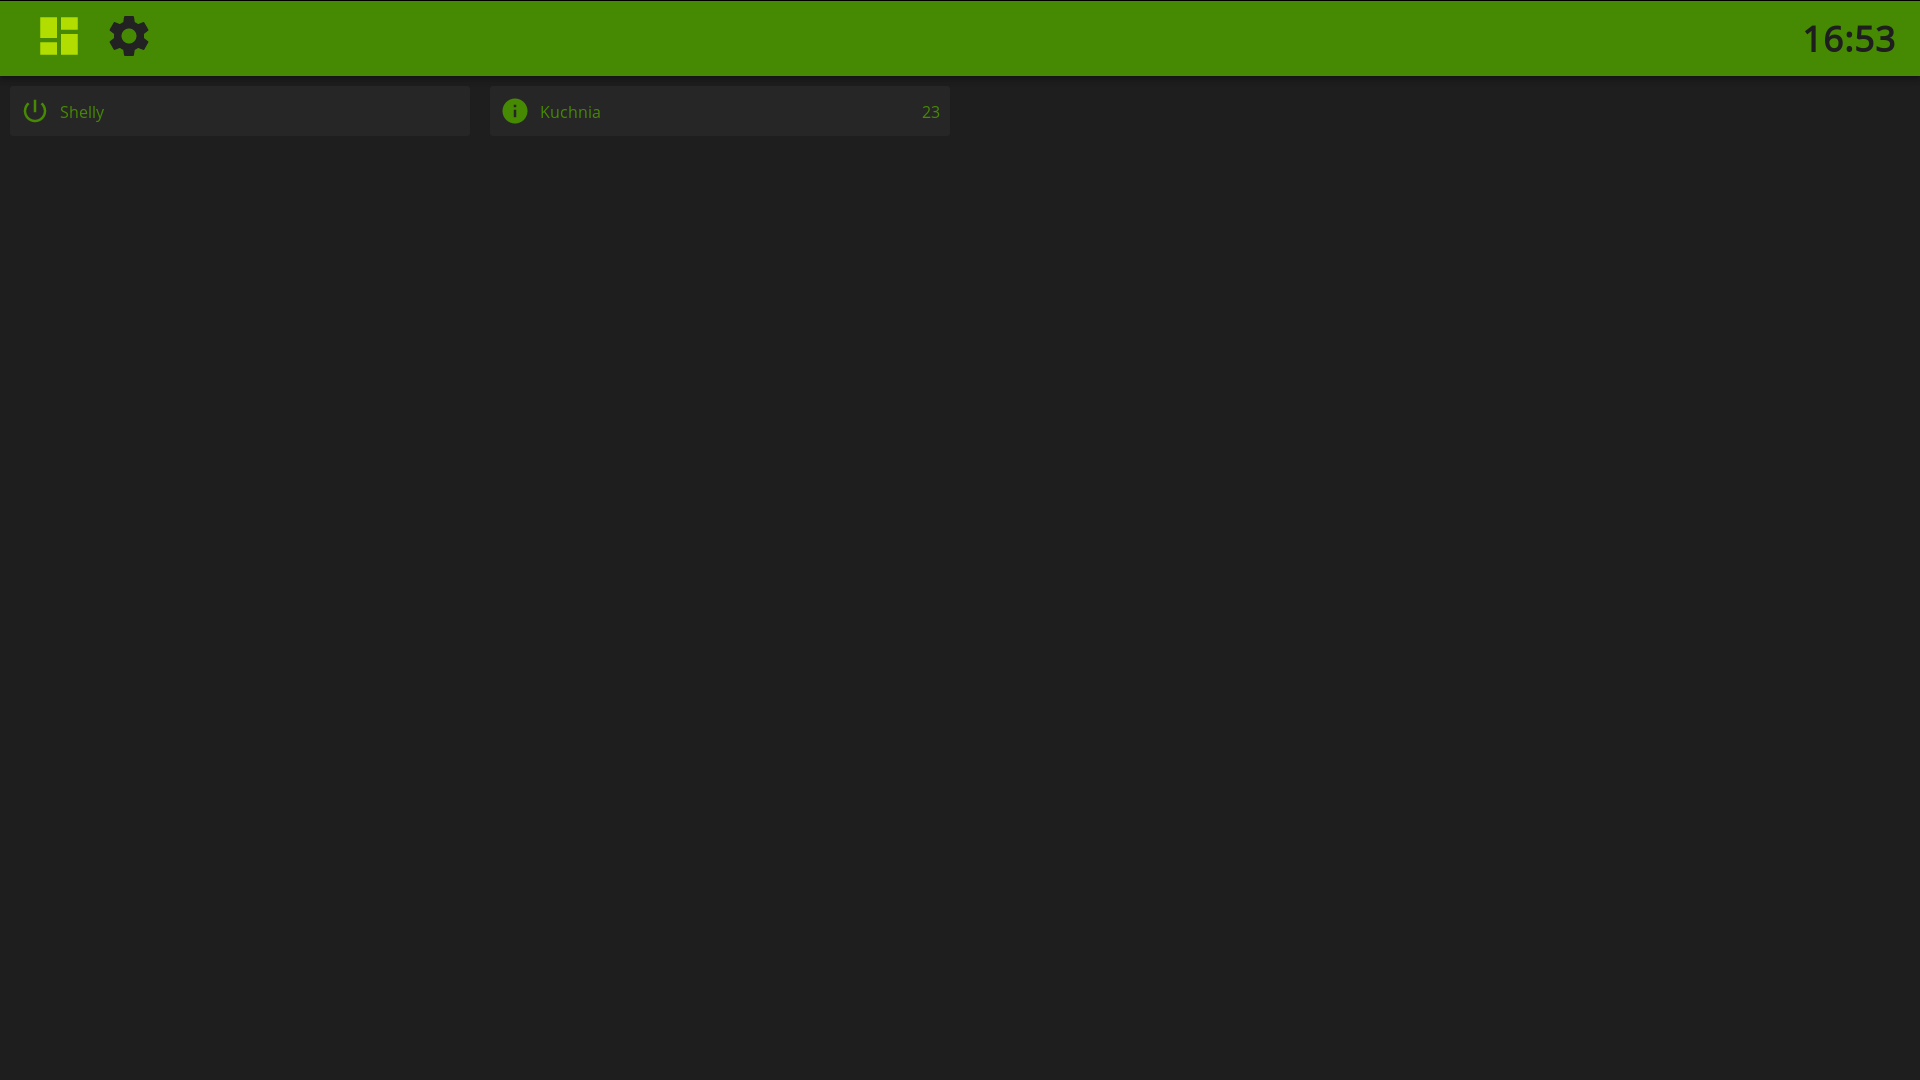
\includegraphics[width=\linewidth]{dashboard.png}
  \caption{Dashboard}
  \label{fig:dashboard}
\end{figure}
\newpage

\subsection{Settings}
Strona służy do konfiguracji naszego systemu. Mamy tu możliwość dodania nowych urządzeń, edycji już istniejących lub wglądu do szczegółów takich jak logi urządzeń.
\begin{figure}[h!]
  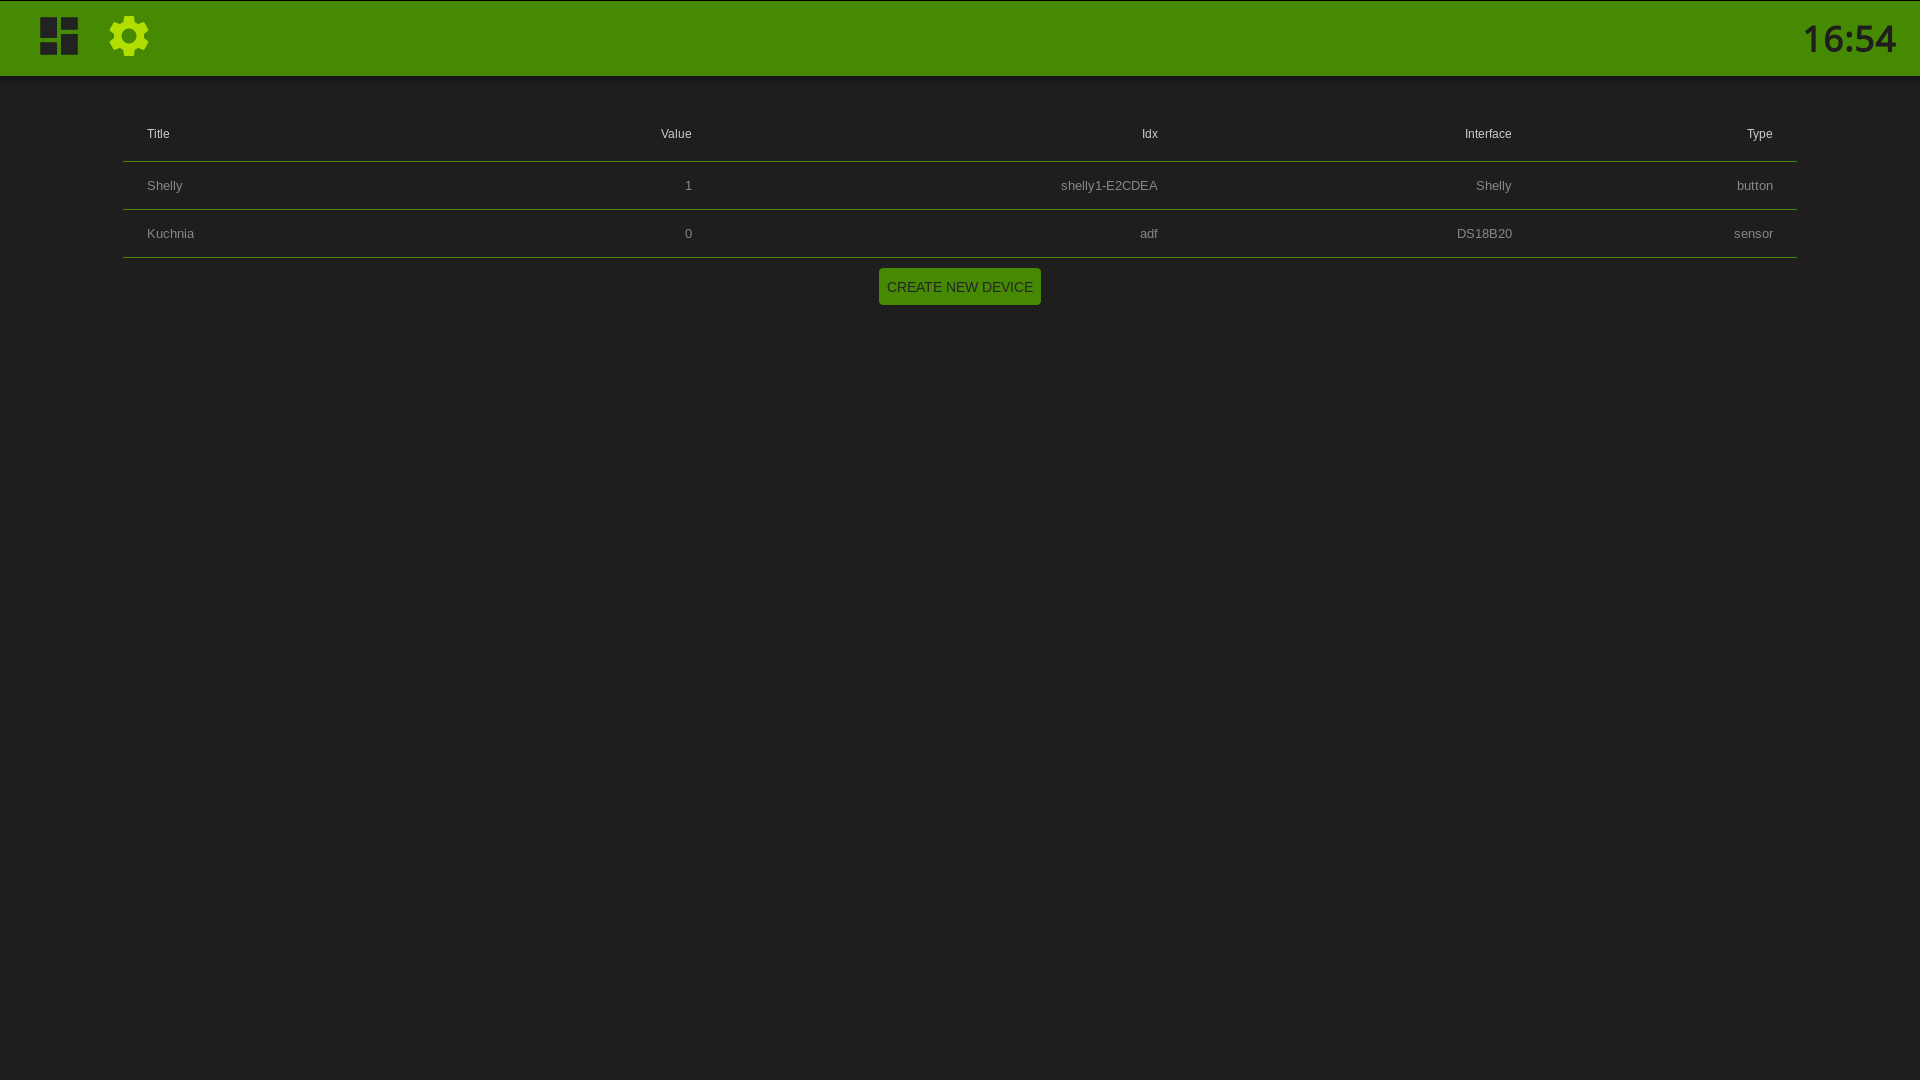
\includegraphics[width=\linewidth]{settings.png}
  \caption{Settings}
  \label{fig:settings}
\end{figure}
\newpage
\section{Serwer}
Serwer jest pośrednikiem między poleceniami użytkownika, a urządzeniami. Jednocześnie zapisuje aktualną konfigurację w bazie danych i trzyma logi. Jest on podzielony na komponenty:
\begin{itemize}
    \item http
    \item baza danych
    \item API do urządzeń
\end{itemize}
Został on napisany w języku javascript i korzysta z transpilera babel-node w celu pracy w wersjach es6+. Serwer posiada dodatkowe testy które sprawdzają działanie niektórych komponentów.
\subsection{HTTP}
Serwer korzysta z obszernego framework'a Express dla języka javascript który pozwala zaimportować cały katalog zawierający stronę \ref{lst:connectPublicCat}. Zbudowana strona jest przechowywana w katalogu \textit{public}. \cite{express}\\
Oprócz tego obsługiwany jest wspominane już zapytanie o port na którym działa websocket \ref{lst:getWSPort}.
Ten krótki kod w \ref{lst:http} pokazuje całą strukturę http w projekcie.
\begin{lstlisting}[columns=fullflexible,caption={http.js}\label{lst:http},language=Java]
export const listen = config => {
    app.get('/websocket_port', (req, res) => {
        res.json({port: config.WS_PORT}) /*!\annotation{lst:getWSPort}!*/
    })
    app.use(express.static(config.HTMLPath)); /*!\annotation{lst:connectPublicCat}!*/
    app.get('/', (req, res) => {
        res.sendFile(`${config.HTMLPath}/index.html`);
    });
    app.listen(config.HTTP_PORT, () => console.log(`http listening on port ${config.HTTP_PORT}`))
}
\end{lstlisting}
\subsection{Baza Danych}
Jako że w założeniach projektu zostało postanowione że powinien on działać na wielu sprzętach to użyta została baza danych relacyjna na silniku SQLite \cite{sqlite}. Sama baza nie jest rozbudowana i zawiera tylko 2 tabele czyli logi i urządzenia. Czas w logach jest typu int mimo że SQLite posiada typ danej timestamp. Powodem tej decyzji jest łatwiejsza integracja ze środowiskiem javascript. \cite{sqlitejs}
\begin{figure}[h!]
  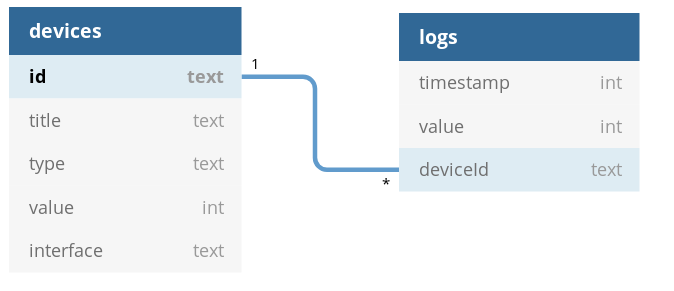
\includegraphics[width=\linewidth]{db.png}
  \caption{schemat bazy}
  \label{fig:db}
\end{figure}

Obsługa bazy danych ma przewidziany osobny moduł w serwerze która upraszcza wiele procesów. Weźmy na przykład funkcję do aktualizacji urządzeń w bazie która została pokazana w \ref{lst:updateDeviceSQL}. Posiada ona tylko jeden argument którym jest urządzenie do zaktualizowania \ref{lst:updateDeviceParameter} Dzięki temu funkcja może być łatwo re-używalna w przypadku integracji nowych urządzeń i pisania do nich komponentów. Funkcja ta buduje komendę SQL \ref{lst:updateDeviceBuildCommand}, a następnie dodaje nowy log w przypadku jak wartość urządzenia uległa zmianie \ref{lst:updateDeviceAddNewLog} (na przykład zmieniła się temperatura).
\newpage
\begin{lstlisting}[columns=fullflexible,caption={edycja urządzenia}\label{lst:updateDeviceSQL},language=Java]
export const updateDevice = (device) => { /*!\annotation{lst:updateDeviceParameter}!*/
	return new Promise(async (resolve, reject) => {
		let command = `UPDATE ${tables.DEVICES} SET`;
		Object.keys(device).forEach(
		    (key)=>key!=='id' && (command+=` ${key}="${device[key]}",`)); /*!\annotation{lst:updateDeviceBuildCommand}!*/
		command = command.slice(0, -1);
		command += ` WHERE id="${device.id}"`;
		const shouldPushLog = await checkIfValueChanged(device);
		if (shouldPushLog) {
			addNewLog(device); /*!\annotation{lst:updateDeviceAddNewLog}!*/
		}

		db.run(command, (err, result) => {
			if (err) {
				console.error(err);
				reject();
			}
			resolve();
		});
	});
};
\end{lstlisting}
Charakter działania wygląda podobnie przy reszcie funkcji z tego modułu dzięki czemu użytkownik tego modułu nie potrzebuje wiedzy o strukturze bazy danych w celu korzystania z niej. 

\subsection{MQTT}
Serwer posiada obsługę MQTT w celu komunikacji z urządzeniami automatyki. W ramach projektu zintegrowany został sterownik przekaźnikowy Shelly1 który jest sterowany właśnie dzięki temu protokołowi. Moduł ten został napisany w osobnym pliku, a program mossquitto pełni funkcję brokera.
\par \ref{lst:initMQTT} pokazuje jedyny spójny element dla każdego modułu wykorzystujący MQTT. W rozdziale 6 została opisana implementacja API w projekcie.

\begin{lstlisting}[columns=fullflexible,caption={inicializacja modułu mqtt}\label{lst:initMQTT},language=Java]
try {
	exec('mosquitto -p 27007', (error, stdout, stderr) => {
		if (error) {
			console.error(error);
		}
	});
} catch (err) { console.log(err) }
\end{lstlisting}
